%% Main-Version Draft
\documentclass[11pt,epsf]{article}
%% -------------------------------
%% |          Packages           |
%% -------------------------------
 \usepackage{amsmath}
 \usepackage{graphicx}
 \usepackage[merge,numbers,compress]{natbib}
 \usepackage[T1]{fontenc}
 \usepackage{booktabs}
 \usepackage{xcolor} 
 \usepackage{xspace}
 \usepackage{dcolumn}
 \usepackage{hyperref}
 \usepackage{caption}
 \usepackage{tabularx}
 \usepackage
 [subrefformat=parens,position=top,skip=-15pt,margin=15pt,justification=justified,singlelinecheck=false]
 {subcaption}

\setlength{\evensidemargin}{0cm}
\setlength{\oddsidemargin}{0cm}
\setlength{\topmargin}{0.00cm}
\setlength{\textwidth}{16.0cm}
\setlength{\textheight}{22.55cm}
\setlength{\headheight}{0cm}
\setlength{\headsep}{0cm}
\setlength{\voffset}{0cm}
\setlength{\paperheight}{27cm}

\renewcommand{\topfraction}{0.8}
\renewcommand{\bottomfraction}{0.5}
\renewcommand{\textfraction}{0.2}
\renewcommand{\floatpagefraction}{0.7}

%% ---------------------------------
%% | ToDo Marker - only for draft! |
%% ---------------------------------
% Remove this section for final version!
\setlength{\marginparwidth}{20mm}

\newcommand{\margtodo}
{\marginpar{\textbf{\textcolor{red}{ToDo}}}{}}

\newcommand{\todo}[1]
{{\textbf{\textcolor{red}{(\margtodo{}#1)}}}{}}

\newcommand{\Pl}{\ell}
\newcommand{\fb}{{\ensuremath\unskip\,\text{fb}}\xspace}
% % new commands for cross referencing
\def\refeq#1{\mbox{(\ref{#1})}}
\def\reffi#1{\mbox{Figure~\ref{#1}}}
\def\reffis#1{\mbox{Figures~\ref{#1}}}
\def\refta#1{\mbox{Table~\ref{#1}}}
\def\reftas#1{\mbox{Tables~\ref{#1}}}
\def\refse#1{\mbox{Section~\ref{#1}}}
\def\refapp#1{\mbox{App.~\ref{#1}}}
\def\citere#1{\mbox{Ref.~\cite{#1}}}
\def\citeres#1{\mbox{Refs.~\cite{#1}}}

\newcommand{\ri}{\mathrm i}

\newcommand{\ie}{\emph{i.e.}\ }
\newcommand{\eg}{\emph{e.g.}\ }

\def\be{\begin{equation}}
\def\ee{\end{equation}}

\newcommand{\qqb}{\ensuremath{q\bar{q}}\xspace}
\newcommand{\PH}{\ensuremath{\text{H}}\xspace}
\newcommand{\Pj}{\ensuremath{\text{j}}\xspace}
\newcommand{\Pp}{\ensuremath{\text{p}}\xspace}
\newcommand{\Pe}{\ensuremath{\text{e}}\xspace}
\newcommand{\Pb}{\ensuremath{\text{b}}\xspace}
\newcommand{\Pq}{\ensuremath{\text{q}}\xspace}
\newcommand{\Pt}{\ensuremath{\text{t}}\xspace}
\newcommand{\Pu}{\ensuremath{\text{u}}\xspace}
\newcommand{\Pd}{\ensuremath{\text{d}}\xspace}
\newcommand{\Ps}{\ensuremath{\text{s}}\xspace}
\newcommand{\Pc}{\ensuremath{\text{c}}\xspace}
\newcommand{\Pg}{\ensuremath{\text{g}}\xspace}
\newcommand{\Pw}{\ensuremath{\text{w}}\xspace}
\newcommand{\PW}{\ensuremath{\text{W}}\xspace}
\newcommand{\PZ}{\ensuremath{\text{Z}}\xspace}
\newcommand{\Pbj}{\ensuremath{\text{j_b}}\xspace}
                                    
\newcommand{\Mt}{\ensuremath{m_\Pt}\xspace}
\newcommand{\MH}{\ensuremath{M_\PH}\xspace}
\newcommand{\MWOS}{\ensuremath{M_\PW^\text{OS}}\xspace}
\newcommand{\MW}{\ensuremath{M_\PW}\xspace}
\newcommand{\MZOS}{\ensuremath{M_\PZ^\text{OS}}\xspace}
\newcommand{\MZ}{\ensuremath{M_\PZ}\xspace}
\newcommand{\Mb}{\ensuremath{m_\Pb}\xspace}
\newcommand{\Gt}{\ensuremath{\Gamma_\Pt}\xspace}
\newcommand{\GH}{\ensuremath{\Gamma_\PH}\xspace}
\newcommand{\GZ}{\ensuremath{\Gamma_\PZ}\xspace}
\newcommand{\GZOS}{\ensuremath{\Gamma_\PZ^\text{OS}}\xspace}
\newcommand{\GW}{\ensuremath{\Gamma_\PW}\xspace}
\newcommand{\GWOS}{\ensuremath{\Gamma_\PW^\text{OS}}\xspace}

\newcommand{\MeV}{\ensuremath{\,\text{MeV}}\xspace}
\newcommand{\GeV}{\ensuremath{\,\text{GeV}}\xspace}
\newcommand{\TeV}{\ensuremath{\,\text{TeV}}\xspace}

\newcommand{\alphas}{\ensuremath{\alpha_\text{s}}\xspace}
\newcommand{\order}[1]{\ensuremath{\mathcal{O}{\left(#1\right)}}\xspace}

\newcommand{\abs}[1]{\left|#1\right|}
\newcommand{\deltar}{\ensuremath{\Delta R}\xspace}

\newcommand{\GF}{\ensuremath{G_\mu}}

\newcommand{\pt}{\ensuremath{p_\text{T}}\xspace}
\newcommand{\ptsub}[1]{\ensuremath{p_{\text{T},#1}}\xspace}
\newcommand{\etsub}[1]{\ensuremath{E_{\text{T},#1}}\xspace}

\renewcommand{\Re}{\mathop{\mathrm{Re}}\nolimits}
\renewcommand{\Im}{\mathop{\mathrm{Im}}\nolimits}

\newcommand{\MVOS}{\ensuremath{M_{V}^\text{OS}}\xspace}%
\newcommand{\GVOS}{\ensuremath{\Gamma_{V}^\text{OS}}\xspace}%

\newcommand{\sq}{\tilde{q}}
\newcommand{\su}{\tilde{u}}
\newcommand{\sd}{\tilde{d}}
\newcommand{\gl}{\tilde{g}}
\def\bom#1{{\mbox{\boldmath $#1$}}}
\newcommand\nn         {\nonumber}
\newcommand{\sul}{\tilde{u}_L}
\newcommand{\scl}{\tilde{c}_L}
\newcommand{\sdl}{\tilde{d}_L}
\newcommand{\ssl}{\tilde{s}_L}
\newcommand{\sur}{\tilde{u}_R}
%\newcommand{\scr}{\tilde{c}_R}
\newcommand{\sdr}{\tilde{d}_R}
\newcommand{\ssr}{\tilde{s}_R}
\newcommand{\stone}{\tilde{t}_1}
\newcommand{\sbone}{\tilde{b}_1}
\newcommand{\sttwo}{\tilde{t}_2}
\newcommand{\sbtwo}{\tilde{b}_2}
\newcommand{\neutone}{\tilde{\chi}^0_1}
\newcommand\sss{\mathchoice%
{\displaystyle}%
{\scriptstyle}%
{\scriptscriptstyle}%
{\scriptscriptstyle}%
}
\newcommand{\newc}{\newcommand}
% \newc{\be}{\begin{equation}}
% \newc{\ee}{\end{equation}}
\newc{\bi}{\begin{itemize}}
\newc{\ei}{\end{itemize}}
\newc{\benu}{\begin{enumerate}}
\newc{\eenu}{\end{enumerate}}
\newc{\bc}{\begin{center}}
\newc{\ec}{\end{center}}
\newc{\bfig}{\begin{figure}}
\newc{\efig}{\end{figure}}
\newc{\qbar}{\bar{q}}
\newc{\go}{\tilde{g}}
\newc{\PB}{\textsc{Powheg-Box}}
\newcommand\matB{{\cal B}}
\newcommand\matR{{\cal R}}
\newcommand\matV{{\cal V}}
\newcommand\matO{{\cal O}}
\newcommand\matF{{\cal F}}

\newcommand{\Recola}{{\sc Recola}\xspace}
\newcommand{\Sherpa}{{\sc Sherpa}\xspace}
\newcommand{\Rivet}{{\sc Rivet}\xspace}
\newcommand{\Amegic}{A\protect\scalebox{0.8}{MEGIC}\xspace}
\newcommand{\Comix}{C\protect\scalebox{0.8}{OMIX}\xspace}
\newcommand{\OpenLoops}{O\protect\scalebox{0.8}{PEN}L\protect\scalebox{0.8}{OOPS}\xspace}
\newcommand{\Njet}{N\protect\scalebox{0.8}{JET}\xspace}
\newcommand{\BlackHat}{B\protect\scalebox{0.8}{LACK}H\protect\scalebox{0.8}{AT}\xspace}
\newcommand{\Gosam}{G\protect\scalebox{0.8}{O}S\protect\scalebox{0.8}{AM}\xspace}
\newcommand{\mocanlo}{{\sc MoCaNLO}\xspace}
\newcommand{\collier}{{\sc Collier}\xspace}
\newcommand{\CutTools}{{\sc CutTools}\xspace}
\newcommand{\OneLOop}{{\sc OneLOop}\xspace}
\newcommand{\madgraph}{{\sc\small MadGraph5\_aMC@NLO}\xspace}
\newcommand{\madgraphbis}{{\sc\small MG5\_aMC@NLO}\xspace}
\newcommand{\rT}{{\mathrm{T}}}
\newcolumntype{.}{D{.}{.}{-1}}
\newcolumntype{d}[1]{D{.}{.}{#1}}

\renewcommand{\vec}[1]{\mathbf{#1}}
\colorlet{tableoverheadcolor}{gray!37.5}
\colorlet{tableheadcolor}{gray!25}
\colorlet{tablerowcolor}{gray!12.5}

\newcommand{\lsim}
{\;\raisebox{-.3em}{$\stackrel{\displaystyle <}{\sim}$}\;}
\newcommand{\gsim}
{\;\raisebox{-.3em}{$\stackrel{\displaystyle >}{\sim}$}\;}
\def\asymp#1{\;\raisebox{-.4em}{$\widetilde{\scriptstyle #1}$}\;}

\newlength{\width}
\newlength{\height}
\newcommand{\brabar}[1]{%
    \settoheight{\height}{\ensuremath{#1}}%
    \settowidth{\width}{\ensuremath{#1}}%
    \makebox[0pt][l]{\ensuremath{#1}}%
    \raisebox{1.26ex}{\scalebox{.3}{\textbf{(}}}%
    \rule[1.41\height]{0.7\width}{0.35pt}%
    \raisebox{1.26ex}{\scalebox{.3}{\textbf{)}}}%
}

% modifications for drafts for drafts
\newcommand{\mpar}[1]{{\marginpar{\hbadness10000%
                      \sloppy\hfuzz10pt\boldmath\bf\textcolor{red}{#1}}}%
                      \typeout{marginpar: #1}\ignorespaces}
\marginparwidth 1.2cm
\marginparsep 0.2cm
\def\draftdate{\relax}
\def\mda{\relax}
\def\mua{\relax}
\def\mla{\relax}
\def\draft{
\def\thtystars{******************************}
\def\sixtystars{\thtystars\thtystars}
\typeout{}
\typeout{\sixtystars**}
\typeout{* Draft mode!
         For final version remove \protect\draft\space in source file *}
\typeout{\sixtystars**}
\typeout{}
\def\draftdate{\today}
\def\mua{\marginpar[\boldmath\hfil$\uparrow$]%
                   {\boldmath$\uparrow$\hfil}\color{black}%
                    \typeout{marginpar: $\uparrow$}\ignorespaces}
\def\mda{\color{red}\marginpar[\boldmath\hfil$\downarrow$]%
                   {\boldmath$\downarrow$\hfil}%
                    \typeout{marginpar: $\downarrow$}\ignorespaces}
\def\mla{\marginpar[\boldmath\hfil$\rightarrow$]%
                   {\boldmath$\leftarrow $\hfil}%
                    \typeout{marginpar: $\leftrightarrow$}\ignorespaces}
\def\Mua{\marginpar[\boldmath\hfil$\Uparrow$]%
                   {\boldmath$\Uparrow$\hfil}\color{black}%
                    \typeout{marginpar: $\uparrow$}\ignorespaces}
\def\Mda{\color{red}\marginpar[\boldmath\hfil$\Downarrow$]%
                   {\boldmath$\Downarrow$\hfil}%
                    \typeout{marginpar: $\downarrow$}\ignorespaces}
\def\Mla{\marginpar[\boldmath\hfil\textcolor{red}{$\Rightarrow$}]%
                   {\boldmath\textcolor{red}{$\Leftarrow $}\hfil}%
                    \typeout{marginpar: $\leftrightarrow$}\ignorespaces}
\overfullrule 5pt
\oddsidemargin 15mm
\marginparwidth 29mm
}

% switch on draft mode
%\draft



\begin{document}

\title{\hfill ~\\[-30mm]
\phantom{h} \hfill\mbox{\small pre-print number if any?}
\\[1cm]
\vspace{13mm}   \textbf{Precise predictions for same sign W-bosons scattering at the LHC}}

\date{}
\author{
Michele Grossi$^{X\,}$\footnote{E-mail:
  \texttt{YY@email.com}},
Alexander Karlberg, 
Mathieu Pellen$^{3\,}$\footnote{E-mail:
  \texttt{mathieu.pellen@physik.uni-wuerzburg.de}},
Giovanni  Pelliccioli, 
Michael Rauch, \\
J\"urgen Reuter,
Vincent Rothe, 
Christopher Schwan,
Pascal Stienemeier,
Marco Zaro.
\\[9mm]
{\small\it
$^1$University X, %
        Institut Y,} \\ %
{\small\it Street X, \linebreak %
        XXXX city, %
        Country}\\[3mm]
{\small\it
$^3$Universit\"at W\"urzburg, %
        Institut f\"ur Theoretische Physik und Astrophysik,} \\ %
{\small\it Emil-Hilb-Weg 22, \linebreak %
        97074 W\"urzburg, %
        Germany}\\[3mm]
}

\maketitle

\begin{abstract}
\noindent
Abstract to be written here.
\end{abstract}
\thispagestyle{empty}
\vfill
\newpage
\setcounter{page}{1}

\tableofcontents
\newpage

\section{Introduction}

The measurements are \cite{Aad:2014zda,Aaboud:2016ffv,Khachatryan:2014sta}.

In the last decade many codes capable of performing VBS simulations have appeared.
Within a network such as VBSCan it is therefore natural to perform 
a quantitative comparison of these codes, both to cross-validate the results and to assess the impact of the different approximations which are used.
In fact, already at LO, when considering the process ${\rm p}{\rm p}\to\mu^+\nu_\mu{\rm e}^+\nu_{\rm e}{\rm j}{\rm j}$ at order $\mathcal O (\alpha^6)$, the various implementations VBS simulations are different.
They differ, for example
by the (non-)inclusion of diagrams with vector bosons in the $s$-channel or by the treatment of interferences between diagrams.
The reason of these differences is that, 
when typical signal cuts for VBS are imposed, these effects turn to be small on rates and distributions.

\section{Definition of the process}

\section{Details of the calculations}

\subsection{Description of the predictions}

In the comparison, the following codes are used: 

\begin{itemize}
 \item The program {\sc Bonsay} consists of a general-purpose Monte Carlo integrator
and matrix elements taken from several sources: Born matrix elements are
adapted from the program {\sc Lusifer} \cite{Dittmaier:2002ap} for the partonic
processes, real matrix elements are written by Marina Billoni, and virtual
matrix elements by Stefan Dittmaier.
One loop integrals are evaluated using the {\sc Collier} library
\cite{Denner:2014gla,Denner:2016kdg}.

  \item {\sc MadGraph5\_aMC@NLO}~\cite{Alwall:2014hca} is an automatic meta-code (a code that generates codes) which makes it possible to simulate any scattering process
      including NLO QCD corrections both at fixed order and including matching to parton showers. It makes use of the FKS subtraction method~\cite{Frixione:1995ms,
        Frixione:1997np} (automated in the module {\sc MadFKS}~\cite{Frederix:2009yq,
        Frederix:2016rdc}) for regulating IR singularities. The computationsof one-loop amplitudes are carried out by switching dynamically between 
        two integral-reduction techniques, OPP~\cite{Ossola:2006us} or Laurent-series expansion~\cite{Mastrolia:2012bu},
        and TIR~\cite{Passarino:1978jh,Davydychev:1991va,Denner:2005nn}. These have been automated in the module {\sc MadLoop}~\cite{Hirschi:2011pa}, which 
        in turn exploits {\sc CutTools}~\cite{Ossola:2007ax}, {\sc Ninja}~\cite{Peraro:2014cba,
        Hirschi:2016mdz}, or {\sc IREGI}~\cite{ShaoIREGI}, together with an in-house implementation of the {\sc OpenLoops} optimisation~\cite{Cascioli:2011va}.\\
        The simulation of VBS at NLO-QCD accuracy can be performed by issuing the following commands in the program interface:
\begin{verbatim}
> set complex_mass_scheme #1
> import model loop_qcd_qed_sm_Gmu #2
> generate p p > e+ ve mu+ vm j j QCD=0 [QCD] #3
> output #4
\end{verbatim}
  With these commands the complex-mass scheme is turned on {\tt \#1}, then the NLO-capable model is loaded {\tt \#2}\footnote{Despite
            the {\tt loop\_qcd\_qed\_sm\_Gmu} model also includes NLO counterterms for computing electro-weak corrections, it is not yet possible to compute such corrections 
        with the current version of the code.}, finally the process code is generated {\tt \#3} (note the {\tt QCD=0} syntax to select the purely-electroweak process)
        and written to disk {\tt \#4}. Because of some internal limitations, which will be lifted in the future version capable of computing both QCD and EW corrections, 
        only loops with QCD-interacting particles are generated.
  \item The {\sc Powheg-Box}~\cite{Alioli:2010xd,Frixione:2007vw} is a framework for mathcing NLO-QCD calculations with parton showers.
It relies on the user providing the matrix elements and Born phase space, but will automaticaly construct FKS \cite{Frixione:1995ms} subtraction terms and the phase space for the real emission.
For the VBS processes all matrix elements are being provided by a previous version of {\sc VBFNLO}~\cite{Arnold:2008rz, Arnold:2011wj, Baglio:2014uba} and hence the approximations used in the {\sc Powheg-Box} are the similar to those used in {\sc VBFNLO}.

  \item The program {\sc Recola+MoCaNLO} is made of a flexible Monte Carlo program dubbed {\sc MoCaNLO}~\cite{MoCaNLO} and the general matrix element generator {\sc Recola} \cite{Actis:2012qn,Actis:2016mpe}.
To numerically evaluate the one-loop scalar and tensor integrals, {\sc Recola} relies on the {\sc Collier} library \cite{Denner:2014gla,Denner:2016kdg},
These tools have been successfully used for the computation of NLO corrections for VBS~\cite{Biedermann:2016yds,Biedermann:2017bss}.

  \item {\sc VBFNLO}~\cite{Arnold:2008rz, Arnold:2011wj, Baglio:2014uba} is a flexible
parton-level Monte Carlo for processes with electroweak bosons. It
allows the calculation of VBS processes at NLO QCD in the VBF
approximation and including the s-channel triboson contribution,
neglecting interferences between the two. Besides the SM, also anomalous
couplings of the Higgs and gauge bosons can be simulated.

  \item {\sc Whizard}~\cite{Moretti:2001zz,Kilian:2007gr} is a multi-purpose
event generator with the LO matrix element generator {\sc O'Mega}. It
provides FKS subtraction terms for any NLO process, while virtual matrix
elements are provided externally by {\sc
OpenLoops}~\cite{Cascioli:2011va} (alternatively, {\sc Recola}~\cite{Actis:2012qn,Actis:2016mpe}
(cf. above) can be used as well). {\sc Whizard} allows to simulate a
huge number of BSM models as well, in particular for new physics in
the VBS channel in terms of both higher-dimensional operators as well as explicit
resonances.

\end{itemize}

The complete comparison of the codes will be published in a separate work. Here, we present some preliminary results obtained at LO ($\mathcal O (\alpha^6)$) and including
NLO QCD corrections at fixed-order $\mathcal O (\alpha^6\alpha_s)$, for the process ${\rm p}{\rm p}\to\mu^+\nu_\mu{\rm e}^+\nu_{\rm e}{\rm j}{\rm j}$.
In Tab.~\ref{tab:wg1_codes} the details of the various codes are reported. In particular, it is specified whether
\begin{itemize}
    \item all $s-$ and $t/u-$channel diagrams that lead to the considered final state are included;
    \item interferences between diagrams are included at LO;
    \item diagrams which do not feature two resonant vector bosons are included;
    \item the so-called non-factorizable (NF) QCD corrections, that is the corrections where (real or virtual) gluons are exchanged between different quark lines,
        are included;
    \item EW corrections to the $\mathcal O (\alpha^5\alpha_s)$ interference are included. These corrections are of the same order as the NLO QCD corrections to
        the  $\mathcal O (\alpha^6$) term.
\end{itemize}
%
\begin{table}
    \footnotesize
    \begin{tabularx}{\textwidth}{c|c|X|X|X|X|X}
        Contact person  &  Code  &  $\mathcal O(\alpha^6)$ $|s|^2/$ $|t|^2/|u|^2$  &  $\mathcal O(\alpha^6)$ interf.  &  Non-res.  &  NF QCD  &  EW corr. to $\mathcal O(\alpha^5\alpha_s)$  \\
        \hline
        \hline
        A. Karlberg  &  {\sc POWHEG}  &  $t/u$  &  No  &  Yes  &  No  &  No  \\
        M. Pellen    &  {\sc Recola+MoCaNLO}  &  Yes  &  Yes  &  Yes  &  Yes  &  Yes  \\
        M. Rauch     &  {\sc VBFNLO}  &  Yes  &  No  &  Yes  &  No  &  No  \\
        C. Schwan    &  {\sc Bonsay}  &  $t/u$  &  No  &  Yes, virt. No  &  No  &  No  \\
        M. Zaro      &  {\sc MG5\_aMC}  &  Yes  &  Yes  &  No virt.  &  No  &  No \\
        V. Rothe     &  {\sc Whizard}  &  Yes  &  Yes  &  Yes  &  Yes  &  Yes \\  
    \end{tabularx}
    \caption{\label{tab:wg1_codes} Summary of the different properties of the codes employed in the comparison.}
\end{table}
%

\subsection{Input parameters}

We simulate VBS production at the LHC, with a center-of-mass energy $\sqrt s = 13 \TeV$. We assume five massless flavours in the proton, and employ the NNPDF~3.0 parton 
density~\cite{Ball:2014uwa}
with NLO QCD evolution (the {\tt lhaid} in LHAPDF6~\cite{Buckley:2014ana} for this set is 260000) and strong coupling constant $\alpha_s\left( \MZ \right) = 0.118$. Since
the employed PDF set has no photonic density, photon-induced processes are not considered. Initial-state collinear singularity are factorised with the  ${\overline{\rm MS}}$ 
scheme, consistently with what is done in NNPDF.\\
We use the following values for the mass and width of the massive particles:
% 
\begin{alignat}{2}
                  \Mt   &=  173.21\GeV,       & \quad \quad \quad \Gt &= 0 \GeV,  \nonumber \\
                \MZOS &=  91.1876\GeV,      & \quad \quad \quad \GZOS &= 2.4952\GeV,  \nonumber \\
                \MWOS &=  80.385\GeV,       & \GWOS &= 2.085\GeV,  \nonumber \\
                M_{\rm H} &=  125.0\GeV,       &  \GH   &=  4.07 \times 10^{-3}\GeV,
\end{alignat}
and renormalise the EW coupling in the $G_\mu$ scheme \cite{Denner:2000bj} where
\begin{equation}
    G_{\mu}    = 1.16637\times 10^{-5}\GeV^{-2}.
\end{equation}
The derived value of the EW coupling $\alpha$, corresponding to our choice of input parameters, is 
\begin{equation}
 \alpha = 7.555310522369 \times 10^{-3}. \\
\end{equation}
We employ the complex-mass scheme~\cite{Denner:1999gp,Denner:2005fg} to treat unstable intermediate particles in a gauge-invariant manner {\bf CHECK THAT ALL CODES USE THE CMS}.\\

Cross sections and distribution are computed within the following VBS cuts inspired from experimental measurements \cite{Aad:2014zda,Aaboud:2016ffv,Khachatryan:2014sta,CMS:2017adb}: 
\begin{itemize}
    \item The two same-sign charged leptons are required to have
        \begin{align}
         \ptsub{\Pl} >  20\GeV,\qquad |y_{\Pl}| < 2.5, \qquad \Delta R_{\Pl\Pl}> 0.3\,.
        \end{align}
    \item The total missing transverse energy, computed from the vectorial sum of the transverse momenta of the two neutrinos in the event,
        is required to be
        \begin{align}
          \etsub{\text{miss}}=p_{\rm T, miss} >  40\GeV\,.
        \end{align}
    \item QCD partons (quark and gluons) are clustered together using the anti-$k_T$ algorithm~\cite{Cacciari:2008gp} with distance parameter $R=0.4$. Jets are required
        to have
        \begin{align}
         \ptsub{\Pj} >  30\GeV, \qquad |y_\Pj| < 4.5, \qquad \Delta R_{\Pj\Pl} > 0.3 \,.
        \end{align}
        On the two jets with largest transverse-momentum the following invariant-mass and rapidity-separation cuts are imposed
        \begin{align}
         m_{\Pj \Pj} >  500\GeV,\qquad |\Delta y_{\Pj \Pj}| > 2.5.
        \end{align}
%         Finally, all jest in the event are required to be separated from charged leptons:
%         \begin{align}
%          \qquad\Delta R_{\Pj\Pl} > 0.3 .
%         \end{align}
    \item When EW corrections are computed, real photons and charged fermion are clustered together using the anti-$k_T$ algorithm with 
        radius parameter $R=0.1$. In this case, leptons and quarks mentioned above must be understood as {\it dressed fermions}. Photons
        which are not combined at this step are clustered with QCD partons to form jets as it is described previously.
\end{itemize}

\section{Fixed order comparisons}

\subsection{Cross sections}

In Tab.~\ref{tab:wg1_LOrates} we report the total rates at LO accuracy obtained with the set-up described above, and in Fig.~\ref{fig:wg1_mjj-llLO} we show the results
for the tagging-jet (left) and lepton-pair (right) invariant-mass distribution. In both case we show the absolute distributions in the main frame of the 
figures, while in the inset the ratio over {\sc VBFNLO} is displayed. For both observables we find 
an excellent agreement among the various tools, which confirms the fact
that contributions from $s-$channel diagrams as well as from non-resonant configurations are strongly suppressed in the fiducial region.
\begin{table}[h!]
    \centering
    \begin{tabular}{c|c}
        Code  &  $\sigma[\rm{fb}]$  \\
        \hline
        \hline
        {\sc Bonsay}  &  $1.5524 \pm 0.0002$ \\
        {\sc MG5\_aMC}&  $1.547 \pm 0.001$  \\ 
        {\sc POWHEG}  &  $1.5573 \pm 0.0003$ \\
        {\sc Recola+MoCaNLO}  &  $1.5503 \pm 0.0003$ \\
        {\sc VBFNLO}  &  $1.5538 \pm 0.0002$ \\
        {\sc Whizard}&  $ 1.5539 \pm 0.0004 $   
    \end{tabular}
    \caption{\label{tab:wg1_LOrates} Rates at LO accuracy within VBS cuts obtained with the different codes used in this comparison, 
    for the ${\rm p}{\rm p}\to\mu^+\nu_\mu{\rm e}^+\nu_{\rm e}{\rm j}{\rm j}$ process.}
\end{table}

\begin{table}[h!]
    \centering
    \begin{tabular}{c|c|c|c}
        Code  &  $\sigma[\rm{fb}]$  \\
        \hline
        \hline
        {\sc Bonsay}  &  $1.3366 \pm 0.0009$  \\
        {\sc MG5\_aMC}&  $1.318  \pm 0.003$  \\
        {\sc POWHEG}  &  $1.334 \pm 0.0003$  \\
        {\sc Recola+MoCaNLO}  &  $1.317 \pm 0.004 $ \\
        {\sc VBFNLO}  &  $1.3531 \pm 0.0003$  \\
    \end{tabular}
    \caption{\label{tab:wg1_NLOrates} Rates at NLO-QCD accuracy within VBS cuts obtained with the different codes used in this comparison, 
    for the ${\rm p}{\rm p}\to\mu^+\nu_\mu{\rm e}^+\nu_{\rm e}{\rm j}{\rm j}$ process.}
\end{table}
At NLO, rates show slightly larger discrepancies, as it can be observed in Tab.~\ref{tab:wg1_NLOrates}. This is most likely due to low dijet invariant-mass configurations, where
$s-$channel diagrams and interferences are less suppressed than at LO, because of the presence of extra QCD radiation.

\subsection{Differential distributions}

\begin{figure}[h!]
   \centering
   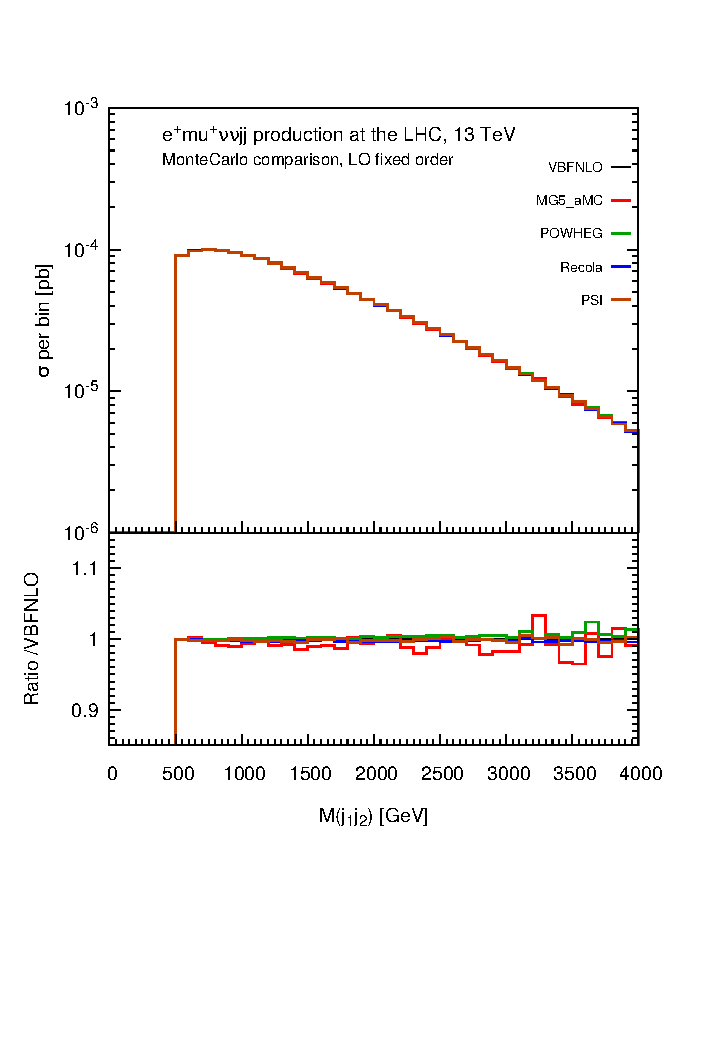
\includegraphics[width=0.49\textwidth,angle=0,clip=true,trim={0.4cm 2.5cm 0.cm 1.cm}]{figures/mjj_LO.pdf}
   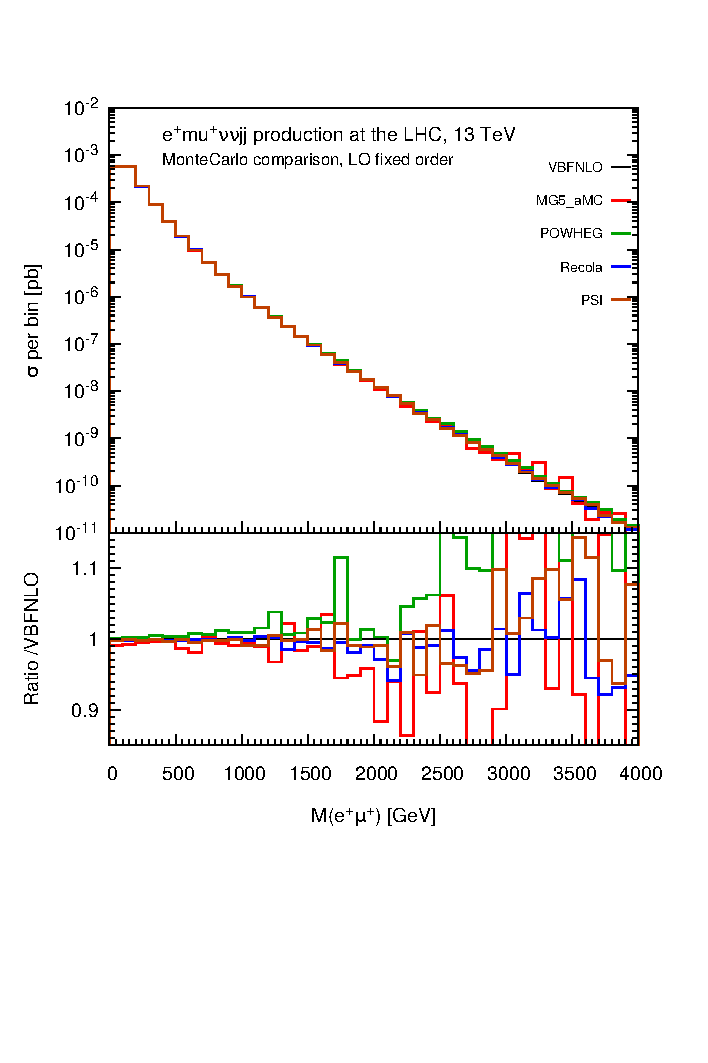
\includegraphics[width=0.49\textwidth,angle=0,clip=true,trim={0.4cm 2.5cm 0.cm 1.cm}]{figures/mll_LO.pdf}
\caption{\label{fig:wg1_mjj-llLO} Invariant-mass of the two tagging jets (left) and of the two leptons (right), at LO accuracy, 
computed with the different codes used in this comparison. The inset shows the ratio over {\sc VBFNLO}.
}
\end{figure}


\section{Influence of the fiducial region}

\section{Matching to parton shower}

\section{Conclusion}

%
\bfig
  \center
%   \includegraphics[width=0.5\textwidth]{figures/ZpT.pdf}
  \caption{Caption of the plot.}
\efig



\section*{Acknowledgements}

We thank ...
Acknowledgement of VBSCAN COST action.

\appendix

\section{Appendix one}


\bibliographystyle{utphys.bst}
\bibliography{article}
\end{document}
